\documentclass{article}
\usepackage{url}
\usepackage{fullpage}
\usepackage{graphicx}
\usepackage[utf8]{inputenc}
\begin{document}
\title{Let's build electrostatic headphones}
\author{Arno Mayrhofer \and Benedikt Becsi}
\maketitle

\tableofcontents

\newpage

\section{Introduction}
\label{s:intro}
The following document will describe the journey to construct your own electrostatic headphones starting with zero, zilch, nada, niente and nichts. In Section \ref{s:tools} we will list the tools required for the building process, which will be followed by a list of materials in Section \ref{s:materials}. The actual construction process is split into five parts, the building of the driver (Section \ref{s:driver}), enclosure (Section \ref{s:driver}), headband (Section \ref{s:headband}) and earpads (Section \ref{s:pads}) with a final assembly in Section \ref{s:assembly}. Finally, the last two chapters will deal with measurements (Section \ref{s:measurements}) and things that we would do differently for the second pair (Section \ref{s:future}).

The whole construction is based on the Head-Fi.org thread \cite{head-fi-diy-thread}, with different and more detailed sources (\cite{electrostatic-hp-design,tcengineering-electrostatic-drivers,ww_1979}) given in the respective sections.

\begin{figure}[htb]
    \centering
    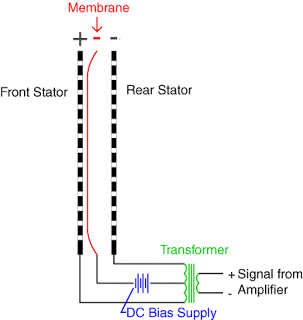
\includegraphics[width=0.5\textwidth]{images/esl_animation.png}
    \caption{Electrical concept}
    \label{f:intro:e-concept}
\end{figure}

The basic electrical concept of a electrostatic headphone can be seen in Fig. \ref{f:intro:e-concept}. An amplifier provides an input signal that is then transformed to yield the desired output voltage that drives the two stators. Additionally, there is a negative DC current that keeps the diaphragm charged.

\section{Required tools}
\label{s:tools}

To build the drivers it is highly recommended that you have access to a good CNC machine. Since we didn't have one of those standing around, we looked for a so called fablab, i.e. a community led workshop for creative projects. We eventually ended up at the Viennese Metalab\footnote{\url{https://metalab.at/}} which gave us access to a heavy duty level CNC machine and an introduction on how to use it by Sebastian Bachmann\footnote{\url{https://www.reox.at/}}, which eased the learning curve significantly. The principal introduction included instructions on how to set up, start and operate the machine and the control terminal, as well as some GGode basics (the programming language that controls the machine's behaviour - more on that in section \ref{s:driver:design:gcode}). Most importantly, as it can be potentially quite dangerous to operate one of those things, it covered security basics, which is definitely the first starting point for anyone new to CNC. Don't skip your tutorial lessons, kids!

Since you might be interested in the budget needed for this, it of course depends on the lab's membership policy - most labs we found had a monthly fee with a minimum subscription period, but we were able to come to an arrangement with a voluntary contribution without binding membership. Most people running those kinds of open creative space are pretty chill, so don't be afraid to ask!

If you can't find a place or plan to work on more DIY-projects in the future, it might be worth it to purchase a CNC mill for yourself or with a group of like-minded people. It's amazing what's going on in the field of affordable, small-scale, DIY and hobby-use CNC in the last couple of years. Here are some links if you're more interested in a purchase:\\
\url{https://www.millrightcnc.com/product-page/millright-cnc-m3-kit-bundle}\\
\url{http://www.makerdreams.it/}\\
\url{https://www.sorotec.de/shop/}\\
\\
Also, some labs require you to buy the wearout parts yourself. You can get CNC parts here:\\
\url{http://cnc-plus.de/}\\
\url{https://www.sorotec.de/shop/}\\
\\
An electric drill was used for the assembly screws and headband construction. The earpads were sewn from hand and as such only thread and needle was required for that. The step up transformer that we built to drive the headphones required a basic electronics lab and in particular a soldering station.

\section{Required materials}
\label{s:materials}
In this section we list all the materials we had to purchase for the headphones and our DIY step-up transformer. We provide you with the links where we bought the materials, but depending on where you live you might find better suppliers yourself.

\begin{enumerate}
    \item 1 mm PCB FR-4 for stators and dust protection spacers:  \url{https://www.conrad.com/ce/en/product/523656/PCB-material-Photo-coating-positive-single-sided-35-m?ref=list}
    \item 0.5 mm PCB for spacers: \url{https://www.conrad.com/ce/en/product/523630/PCB-material-Photo-coating-positive-single-sided-35-m?ref=list}
    \item 3 $\mu m$ Mylar (for diaphragm): \url{https://www.ebay.com/itm/Electrostatic-Speaker-Membrane-Dupont-Mylar-C-3um-40M/172781729300?epid=666335680&hash=item283a97f614:g:jg0AAOSwrklVPe61} (with that, you should have all your mylar needs covered for years to come!)
    \item 1 $\mu m$ Mylar (for dust protection): \url{https://www.freeflightsupplies.co.uk/index.php/products/lightweight-covering-materials}
    \item Anti-static display cleaner for diaphragm coating: \url{https://www.conrad.com/ce/en/product/995207/DataFlash-DF1620-Content-250-ml?ref=searchDetail}
    \item Acrylic spray for insulating the stators: \url{https://www.conrad.com/ce/en/product/1198455/Acrylic-paint-Revell-Black-matt-08-Spray-can-100?ref=searchDetail}
    \item Thin and stretchy artificial leather for the earpads and headband (should be available in a textile shop)
    \item Wood for the enclosure and headband, several boards with 4mm and 10mm thickness; we used lime and spruce
    \item Metal rods (3mm welding rods) for the headband
    \item 3 cm acoustic foam (pads and headband)
    \item Cable plus connectors
    \item Screws for the assembly (2,5 x 20 mm)
    \item Clear varnish or glaze for wood finish
    \item Two-component glue: \url{https://www.conrad.com/ce/en/product/478703/UHU-Plus-Schnellfest-Two-component-adhesive-45700-35-g?ref=list}
    \item Contact glue for gluing the membrane to the stators and the earpads: \url{https://www.conrad.com/ce/en/product/631802/UHU-greenit-Contact-adhesive-45401-650-g?ref=searchDetail}
    
\end{enumerate}
Here's a more comprehensive list of material suppliers: \url{http://www.head-fi.org/t/826032/electrostatic-ear-speaker-diyers-suppliers-list}
\\
\\
Materials needed for the amplifier:
\begin{enumerate}
    \item 4 Audio transformers 6V - 230V (OEP N35A002F) \footnote{\url{https://uk.rs-online.com/web/p/audio-transformers/2106475/}}
    \item 1 Power transformer 230V - 230V (Triad Magnetics FP230-25) \footnote{\url{https://eu.mouser.com/search/ProductDetail.aspx?r=553-FP230-25}}
    \item 2 1 Ohm wirewound resistors \footnote{\url{https://eu.mouser.com/search/ProductDetail.aspx?r=71-RS0101R000FE73}}
    \item 6 1kV diodes \footnote{\url{https://eu.mouser.com/search/ProductDetail.aspx?r=625-RGP10M-E3}}
    \item 2 10 MOhm resistors \footnote{\url{https://eu.mouser.com/search/ProductDetail.aspx?r=594-SFR25H0001005JR5}}
    \item 6 10 nF capacitors \footnote{\url{https://eu.mouser.com/search/ProductDetail.aspx?r=75-564R30GAS10}}
    \item 1 3.9 kOhm resistor \footnote{\url{www.aliexpress.com}}
    \item Power cord plus plug
    \item Cables
    \item Test circuit board
\end{enumerate}

\section{Building the driver}
\label{s:driver}

\subsection{Design of the stators and spacers}
\label{s:driver:design}
Diameter of the holes (2mm) should not be larger than the distance from stator to spacer. The holes in the stator should not cover the whole stator. Instead there should be a perimeter that acts as an air damper and avoids resonance frequencies in the upper midrange or lower treble. The size of the diaphragm is quite important as low frequencies require a large diaphragm surface. The active area should have a diameter of about 80 mm. The ratio of spacer thickness to diaphragm width should not be larger than 1:120 to avoid contact between stator and diaphragm. Lowering the bias voltage can help with very large ratios. Open area of the stators should be around 40\% in order to avoid issues with stability of the stator.

When drilling holes on the stator the feed rate should be at around 3600 mm/min.  For routing and cutting, it should be slowed down to around 1800 - 2400 mm/min.

In order to protect the diaphragm a dust and sweat protection needs to be used. This dust cover will be made from crumpled Mylar and will be located on the same side as the coating of diaphragm.

\url{http://www.head-fi.org/t/498292/my-diy-electrostatic-headphones/660#post_8897170} -> Design pictures of the Orpheus clones; apparently this design lacks some bass punch, maybe increase non-holed perimeter for improvements? Later on it is proposed to decrease the width a bit to improve stability. This would yield the dimensions of 110 x 74 mm (open area of 104 x 74 mm of orpheus clone).

\url{http://www.head-fi.org/t/498292/my-diy-electrostatic-headphones/1155#post_10142154} -> potential improvement of stability by making a hole in the center of the stators (one additional advantage: it's easier to detect issues with the diaphragm as it can be examined visually)

The edges of the spacers need to be sanded down a bit in order to avoid copper dust on the sides and spurious electrical contacts. Holes should be de-burred from copper.

Do not mirror the stators so that the drilling always goes away from the diaphragm (drill pushes small bits of material on the outside) TODO REPHRASE

\subsubsection{Gcode creation}
\label{s:driver:design:gcode}
Inner ellipse: 55 x 37, outer: 65 x 47. Radius of holes: 1mm, multiplicator: 39 in x and 26 in y direction with distance 0.8421 and 0.88 in those directions, respectively.

Current setup:

\begin{itemize}
    \item FreeCad to make the designs -> export as svg
    \item Inkscape to place the svgs correctly \& create stator holes -> export as svg
    \item Makercam.com to create gcode.
\end{itemize}

CNC Drills:

\begin{itemize}
    \item 2mm drill for pcb
    \item 2mm end mill for pcb (diamond coated)
    \item 6mm drill for wood 2-flute
    \item 2mm drill for wood 2-flute
\end{itemize}

Ordered via \url{www.cnc-plus.de} and \url{www.sortec.de}.

\subsection{Etching the stators}
\label{s:driver:etching}
Etching the PCB board ensures that electrical contacts are only where they absolutely need to be. Furthermore, having less copper surface will result in a reduced capacitance and they will be easier to drive because of that. Toner transfer can be used to define the areas that should not be etched. After etching the stators can be protected by spraying thin layers of Acrylic paint on the copper (flat not glossy paint). This insulation avoids degradation of the copper surface and potential shorts when dust is present between the diaphragm and the stators. A small area needs to be left open so that wires can be soldered onto the stators.

\url{http://www.instructables.com/id/Stop-using-Ferric-Chloride-etchant!--A-better-etc/}

Etching is achieved by using 2 parts Hydrogen Peroxide (3\%) with 1 part Hydrochloric acid (30\%). Most PCBs have a photosensitive coating that needs to be removed for this to work. The etching can be achieved by using a paintbrush to apply the solution to the desired location. The copper will be taken away rather quickly and the solution will turn greenish.

\subsection{Tensioning the Mylar diaphragm}
\label{s:driver:tension}
Mylar with 3 $\mu m$ thickness is used to create the diaphragm. Thinner Mylar will cause a lack of bass, while thicker one will cause problem in treble and mids. The tensioning should be high enough as otherwise the diaphragm will collapse onto a stator but also low enough in order to not reduced the bass.
Different ways of tensioning the Mylar:
\begin{enumerate}
    \item With weights on the side
    \item Using a bicycle tire and inflating it
    \item Using tape to stretch it
\end{enumerate}
\begin{figure}[htb]
    \centering
    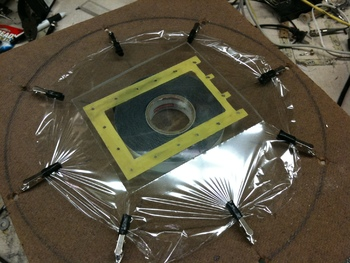
\includegraphics[width=0.5\textwidth]{images/mylar-tension-weight.png}
    \caption{A Mylar tensioning rig using weights}
    \label{f:driver:tension:weight}
\end{figure}
\begin{figure}[htb]
    \centering
    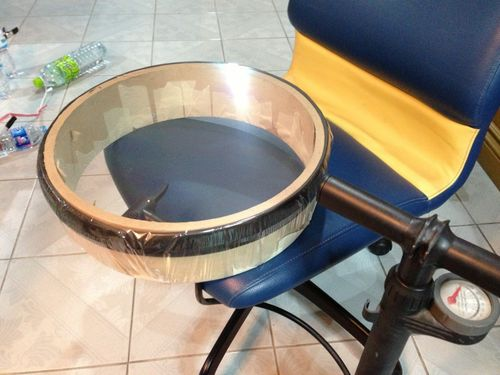
\includegraphics[width=0.5\textwidth]{images/mylar-tension-tire.png}
    \caption{A Mylar tensioning rig using an inflatable tire}
    \label{f:driver:tension:tire}
\end{figure}
\url{http://www.head-fi.org/t/498292/my-diy-electrostatic-headphones/720#post_9217468} -> Orpheus clone tensioning; weights should be larger between 0.8 and 1.0 kg. Preferred option

\url{http://www.head-fi.org/t/498292/my-diy-electrostatic-headphones/1095#post_9907534} -> tire tensioning jig.

Before putting it on the glass (and before coating) clean it with Acetone. To cut the Mylar after glueing use a soldering iron. Ensure there is no Mylar beyond the edges. The stators might warp slightly but this should be ok when assembling the driver.

Make sure the diaphragm is very well glued to the stator. The contact cement is applied to the spacer which is allowed to sit for 3-5 minutes. After that the spacer is put on the Mylar and a bond will be created immediately. A good contact can be achieved by running the finger along the spacers several times so that the glue is everywhere in contact with the spacer. See \url{http://www.head-fi.org/t/498292/my-diy-electrostatic-headphones/1215#post_10400583}

After glueing the Mylar onto the spacers knock them on the side of a table to check that the sound of both diaphragms is similar. If not, a hot air gun can be used to tension the one with a looser sound.

Tension is sufficient if wrinkles on the Mylar vanish during the procedure, corresponding to about 0.5\% of displacement. The two diaphragms need to be glued on the same mylar film so that the tension is the same on both sides.

\url{http://www.head-fi.org/t/498292/my-diy-electrostatic-headphones/1770#post_11440100} idea on how to identify the correct tension of the diaphragm by checking the free-air resonance frequency (should be between 100 and 200 Hz) using a white noise generator on one side and a microphone on the other.

\subsection{Coating the diaphragm}
As Mylar is not conductive an additional coating is required so that it can be charged. It basically should act as if it was a capacitor, so a coating that is conductive and has a high resistivity is ideal. Coating agents are:
\begin{enumerate}
    \item Staticide 6300 (anti static cleaner for monitors)
    \item Licron antistatic spray
    \item Swash Floor cleaner
\end{enumerate}
Coating is achieved by applying a small drop of Staticide onto the diaphragm and then spreading it with a sponge or microfibre cloth (lint free!). After it dries clean wipe the surface again with a dry lint free cloth.

Thread about coating: \url{http://www.diyaudio.com/forums/planars-exotics/109789-esl-diaphragm-coating.html}

Is this Staticide a gel?

\subsection{Assembly}
\label{s:driver:assembly}
Synthetic rubber glue (contact cement, UHU Greenit, alternatives: UHU Por, 3M 4693) is used to glue the diaphragm to the spacers. The dust protection screen must also be placed on some spacers (1mm thickness PCB) and must not be in contact with the stators. 1 $\mu m$ Mylar is crumpled and then stretched somewhat so that it doesn't touch the stators when on the spacer. This yields an ideal acoustically transparent material for dust protection. Normally, no dust cover is used on the outside. As no sweat protection is required on this side a very fine cloth could be used if needed. Only one spacer is glued to the diaphragm. This spacer will be the one facing the outside. The spacer on the inside will have the copper side in contact with the coated diaphragm and will be the one with the electrical contact to the DC bias voltage.
\begin{figure}[htb]
    \centering
    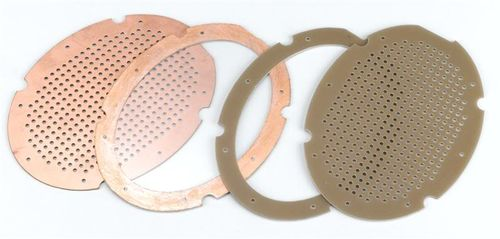
\includegraphics[width=0.5\textwidth]{images/arrangement.png}
    \caption{Arrangement and orientation of stators and spacers (missing the dust protection spacer and film)}
    \label{f:driver:assembly:arrangement}
\end{figure}

Plastic screws are used to assemble the driver unit.

Adhesive tape (masking tape) and pressurized air can be used to clean the dust of the diaphragm and stators. A magnifying glass should be used for checking cleanliness.

The driver can be tested by hooking it up to the amp and leave it as is for 3 to 4 hours without playing any music. The diaphragm should not be sucked to one side during this.

%\subsection{TODO}
%\begin{enumerate}
%    \item What does it mean to bias the headphone for a certain voltage?
%    \item What is used to coat the diaphragm? Coating is done with a wet sponge maybe.
%    \item How much does the Mylar need to be stretched ($< 1\%$)? About 0.5 \% seems reasonable
%    \item How to do accurate etching and what chemicals should be used? FeCl or HCl are options
%    \item How can the surface resistance of the diaphragm be measures? Simply measure at opposite sides? Check multimeter capabilities as it might not be able to measure resistance in the GOhm range. Try to find alternative ways of measuring resistance if that is the case. Resistance should be around 10 - 100 MOhm per square (cm ?). \url{https://dannyelectronics.wordpress.com/2016/01/28/the-nano-ammeter-you-already-have/} shows a way to measure small currents
%\end{enumerate}

\subsection{Potential improvements}
\begin{enumerate}
    \item Drill holes with two different sizes to get a larger hole to surface area ratio
    \item A space filling curve could be used to further reduce the copper on the stators
\end{enumerate}

\section{Building the enclosure}
\label{s:enclosure}
Wooden enclosures are potentially problematic as they can attract moisture which can cause electrical leakage. Sennheiser uses varnish on the outside of their wooden cups but none on the inside. It is possible to use a plastic O-ring to avoid direct contact between the wood and the driver.

\section{Building the headband}
\label{s:headband}

\url{http://www.head-fi.org/t/498292/my-diy-electrostatic-headphones/675#post_8943826}

Headband can be made out of a metal ruler and then covered with leather \url{http://www.head-fi.org/t/498292/my-diy-electrostatic-headphones/2385#post_13037825}.

\section{Building the earpads}
\label{s:pads}
The earpads should be thick enough so that the bass is powerful and deep enough.
\begin{figure}
\centering
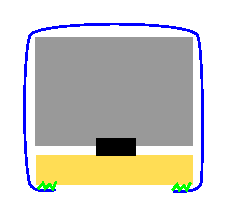
\includegraphics[width=0.3\textwidth]{images/earpad.pdf}
\caption{Earpad cut-through; materials: wood (yellow), foam (grey), screw nut (black), artificial leather (blue), contact cement (green)}
\label{f:pads:cut}
\end{figure}
The earpad is based on a wooden ellipse with 4mm thickness that was also manufactured using the CNC. After we had the full enclosing together we put the front and the back of the enclosing together with this ellipse to drill four holes for the assembly. The screw nuts were glued to the inside of the ellipse using copious amounts of epoxy. A schematic of the earpad can be seen in Fig. \ref{f:pads:cut}. After the glue has hardened (see your glue for the time, for ours it was about 24h) we loosened the screws and disassembled everything. The next step consisted of cutting the same ellipse from acoustic foam with 3cm thickness.

The leather cover is made from a thin and stretchy synthetic leather. It's made of two parts, a rectangular one with dimension 4 x 32 cm and an elliptic one which is of the same size as the wooden ellipse of the pad plus 1 cm inside and 3 cm on the outside. The rectangular patch is sewn on the inside of the ellipse and then it's wrapped over the foam and the wooden pad connector. The leather is glued to the wood using the contact cement that was also used to glue the diaphragm to the spacers. Finally, we also glued a mesh to the wood so that the ears cannot get in touch with the dust protector.

\begin{figure}
\centering
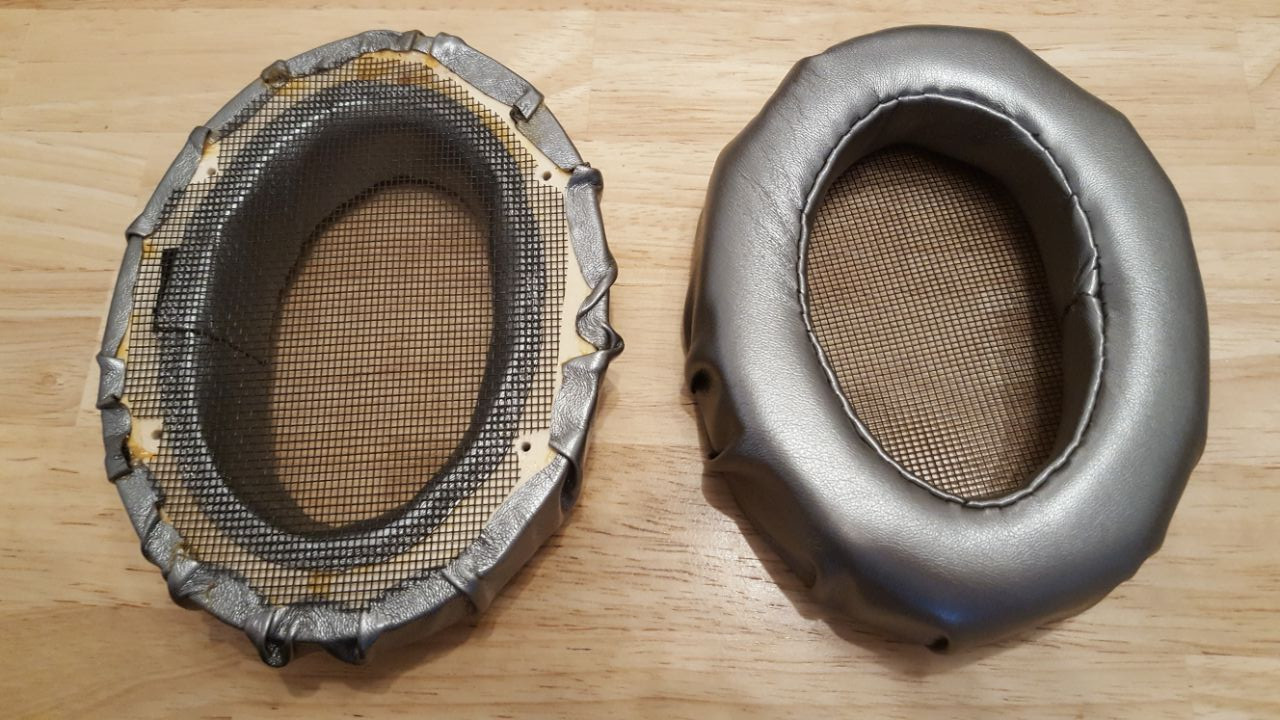
\includegraphics[width=0.7\textwidth]{images/earpads_final.jpg}
\caption{Final earpads}
\label{f:pads:final}
\end{figure}

%\subsection{Potential improvements}
%\begin{enumerate}
%    \item Material should be leather on the inside. Sennheiser HE60/90 has fabric in contact with head, leather everywhere else. This makes it more comfortable
%    \item It might be worth having harder foam on the inside as it will reduce resonances. Obviously this needs to be balanced to ensure comfort.
%    \item Is it possible to make individual ear pads? Would allow for the use of harder materials. Moving your mouth changes the geometry so one would need to be careful.
%\end{enumerate}
%Post on ear pads: \url{http://www.head-fi.org/t/498292/my-diy-electrostatic-headphones/660#post_8930271}. Inner diameter of Orpheus earpads is 45mm x 90mm.

\section{Assembly}
\label{s:assembly}

\subsection{Cable}
The cable that connects the headphone with the step up transformer consists of three about 3m long litz wires ($0.14mm^2$)that were braided together. One side was soldered directly onto the stators and one spacer whereas the other side was fitted with banana plugs to connect the headphones to the transformer.

While this might not be the perfect solution in terms of elegance and signal transmission it was a inexpensive and functional way to make the headphones sing.

Alternatives include replacement cables for KOSS headphones. Apparently an extension cable for the ESP-950 headphone should do the trick. \footnote{\url{https://www.head-fi.org/threads/my-diy-electrostatic-headphones.498292/page-51#post-9325470}}

%Cables should be doubly insulated to withstand the high voltage. DIN plugs are used by many for electrostatic headphones but it might not be safe due to the high voltages, same for XLR. Ribbon cables rated for high voltages are recommended.
%\begin{enumerate}
%    \item Cable building (low capacitance)
%    \item Connector building: need 6 pins ideally (3 for each side, for front and rear stator as well as one for the diaphragm DC voltage)
%\end{enumerate}

\section{Amplifier}
\label{s:amp}
Due to the requirement of a continuously charged diaphragm and the high voltage requirements of the stators a dedicated amplifier is required for electrostatic headphones.
\begin{figure}[htb]
    \centering
    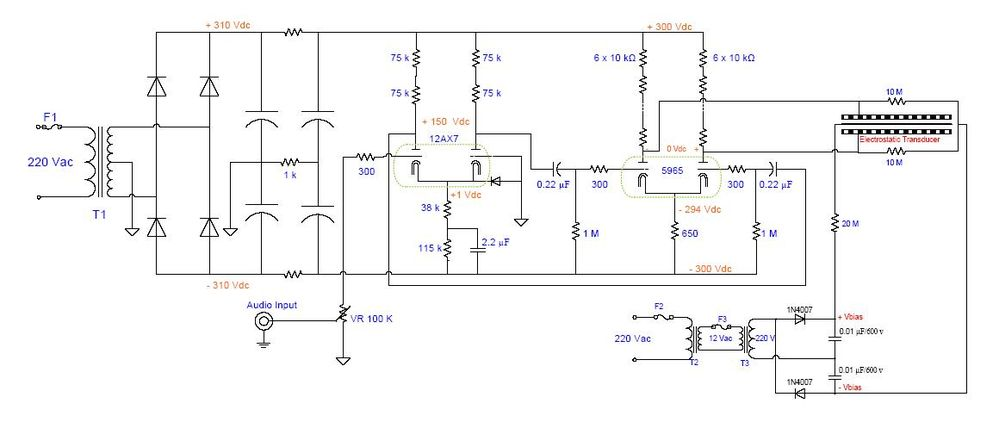
\includegraphics[width=0.5\textwidth]{images/wachara-amp.png}
    \caption{Amplifier design by Wachara C.}
    \label{f:amp:wachara}
\end{figure}
A discussion on this amplifier design can be found on Head-fi.org \footnote{\url{http://www.head-fi.org/t/498292/my-diy-electrostatic-headphones/720#post_9182523}}. However, to not make out lives too difficult we decided against building a full amplifier. Instead we opted to construct a step up transformer based on the designs of Charlie Mimbs \footnote{\url{https://jazzman-esl-page.blogspot.co.at/2010/01/update-new-toroidal-step-up.html}}.

A note of warning before we continue with the details. We will be dealing with electronic equipment in the following which can cause serious injury or death so make sure you have a good understanding of what you are doing and follow proper safety procedures.

Since we are not building a speaker we opted for a toned down version of Charlie's step up that would only lead to 580 volts at the diaphragm. A circuit diagram can be seen in Fig. \ref{f:amp:step-up} that was copied from circuitjs \footnote{\url{http://lushprojects.com/circuitjs/circuitjs.html}}.

\begin{figure}[htb]
    \centering
    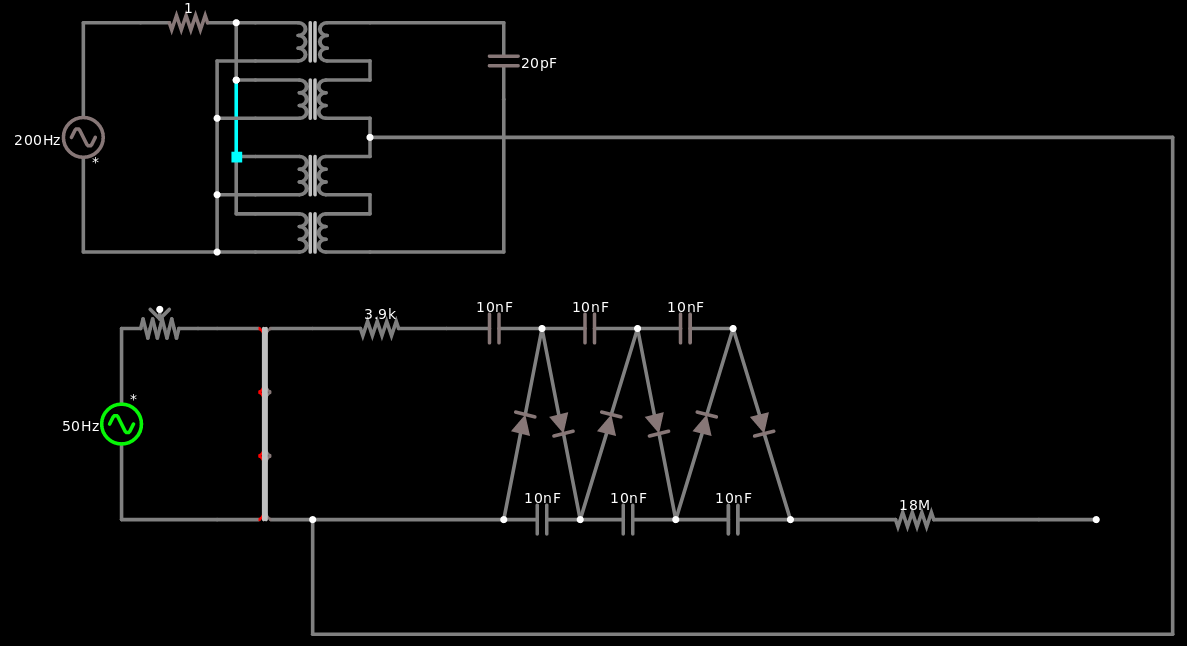
\includegraphics[width=0.7\textwidth]{images/step-up-transformer.png}
    \caption{Step up transformer: circuit diagram}
    \label{f:amp:step-up}
\end{figure}

The final step-up transformer can be seen in Fig. \ref{f:amp:step-up-real}. As can be seen, we did not put it in a nice enclosing and this will also be part of next years project. The step-up transformer is divided in three parts, the blue and yellow part are the transformers for the left and right stators, respectively. Each of these section consists of one 1 Ohm resistor and 2 audio transformers from 6 V to 230 V. The OEP transformers that we used (see Section \ref{s:materials}) were connected on the B-D and 1-4 pins. This yields a 4000k to 95k winding ratio. The two transformers are connected in series and the output side is connected to the step-up part of the transformer as can be seen in Fig. \ref{f:amp:step-up}. Note that in the circuit diagram only one of these stator sections is depicted.

\begin{figure}[htb]
    \centering
    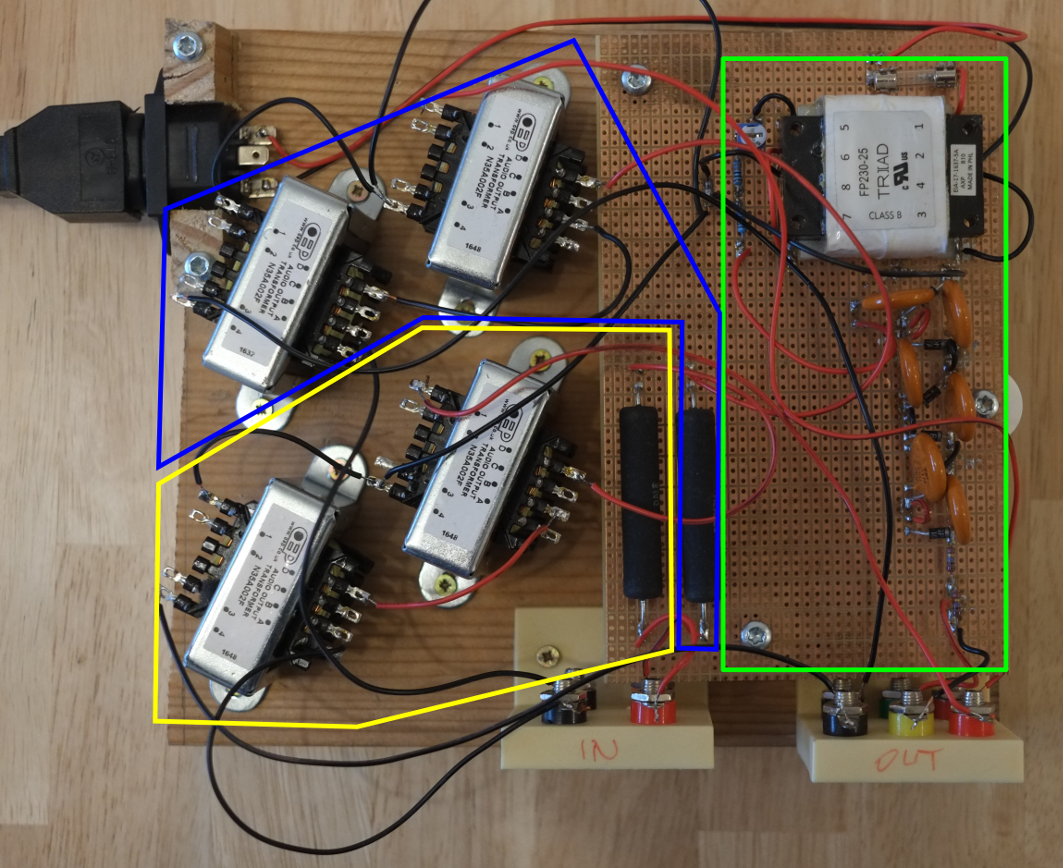
\includegraphics[width=0.95\textwidth]{images/step-up-real-top.png}
    \caption{Step up transformer from the top}
    \label{f:amp:step-up-real}
\end{figure}

The green part in Fig. \ref{f:amp:step-up-real} corresponds to the lower part in the circuit diagram (Fig. \ref{f:amp:step-up}) and is responsible for converting the 230 V, 50 Hz AC input to a 580 V DC current. The AC input was connected to the Triad power transformer including a 250mA fast blow fuse. On the output side a 3.9 kOhm resister is put before the actual step-up ladder that can be seen in the circuit diagram. This ladder consists of 6 10 nF capacitors and 6 diodes to rectify the AC current. At the end of this ladder a 18 MOhm resistor is put before the connection to the diaphragm is made. Note that we made only one step-up ladder that is connected to both left and right diaphragms.

Note that when operating the headphone its component will be charged and this charge will persist even if power to the transformer has been shut down. It is necessary to discharge all components before disassembly which can be achieved by leaving the power cord connected after shutdown and using the ground connection of the power cord. We hooked up a cable to the ground connection and discharge all outgoing ports by touching them briefly with this cable.

%Check if it is possible to add a voltage regulator to try out different bias voltages easily \url{http://www.head-fi.org/t/498292/my-diy-electrostatic-headphones/1560#post_10959595}.
%
%Amp safety: \url{http://www.head-fi.org/t/498292/my-diy-electrostatic-headphones/1455#post_10705917} and \url{http://www.head-fi.org/t/498292/my-diy-electrostatic-headphones/1470#post_10706261}
%
%Check design in article \cite{ww_1979} and \cite{verwaal_2011}.
%
%Turn ratio should be at least around 1:40.
%
%\url{http://www.head-fi.org/t/498292/my-diy-electrostatic-headphones/2415#post_13059527} pdf with some links and amp designs

\section{Measurements}
\label{s:measurements}

As part of the current build we did not perform any measurements and this will become a topic for the future. The head-fi thread suggests to perform measurements with and without seal. The latter should give a peak at around 200 Hz which is the free-air resonance frequency. This frequency should be lower than 150 Hz for a good bass response.

\section{What to do different in the future}
\label{s:future}

Allow for a little space between enclosing and driver.

Shrink wrapped cable with proper xlr connector.

Earpad made out of three pieces (2 rectangular ones and one ellipse).

\subsection{Closed headphones}
\label{s:future:closed}

Materials used for damping included felt, wool or other acoustically semi-transparent materials. Some also coat the inside of the enclosure with Bitumen.

\section{Collaboration \& License}
This work is licensed under a Creative Commons Attribution-ShareAlike 4.0 International License \footnote{\url{http://creativecommons.org/licenses/by-sa/4.0/}}. The official repository for this guide can be found on github.com \footnote{\url{https://github.com/Azrael3000/headphone-guide}}. There is an issue tracker available if you do not know how to work with \LaTeX and git. We very much jumped into this venture without prior knowledge of a lot of things that we had to tackle. Because of this there might very well be mistakes in this guide or in our approach that we are happy to learn about. So do get in touch with us if you have any remarks and want to help us improve this document. We plan to build version 2 of the headphones in 2018 and with this we will also update and improve this guide.

\section{Appendix}
\label{s:app}

\subsection{Circuit diagram for circuitjs}
\label{s:app:circuit}
\begin{verbatim}
$ 13 0.000005 146.80153516788286 47 120 28
v 448 512 448 352 0 1 50 230 0 1.5707963267948966 0.5
c 720 352 800 352 0 1e-8 -121.77903323034391
w 608 512 608 608 0
w 608 512 768 512 0
d 768 512 800 352 1 0.805904783
d 800 352 832 512 1 0.805904783
d 832 512 880 352 1 0.805904783
d 880 352 912 512 1 0.805904783
d 912 512 960 352 1 0.805904783
d 960 352 1008 512 1 0.805904783
c 800 352 880 352 0 1e-8 -188.52952984256655
c 880 352 960 352 0 1e-8 -148.45206709826482
c 768 512 832 512 0 1e-8 -188.38552969850758
c 832 512 912 512 0 1e-8 -148.28294550190276
c 912 512 1008 512 0 1e-8 -133.83898987162684
r 1008 512 1216 512 0 18000000
w 1216 512 1264 512 0
w 608 608 1328 608 0
v 416 96 416 288 0 1 200 6 0 0 0.5
T 560 96 656 112 0 4 20 -0.0002165438913044398 0.000008783616360946498 0.999
T 560 176 656 144 0 4 20 0.00021654389130444608 -0.000008783616360946477 0.999
T 560 240 656 208 0 4 20 0.00021654389130505795 -0.00000878361636097594 0.999
T 560 288 656 256 0 4 20 0.00021654389130505323 -0.000008783616360975917 0.999
w 656 128 656 144 0
w 656 240 656 256 0
r 544 96 464 96 0 1
w 544 96 560 96 0
w 544 208 560 208 0
w 544 144 560 144 0
w 544 208 544 256 0
w 544 256 560 256 0
w 544 208 544 144 0
w 544 144 544 96 0
w 560 128 528 128 0
w 528 128 528 176 0
w 528 176 560 176 0
w 528 176 528 240 0
w 528 240 560 240 0
w 560 288 528 288 0
w 528 288 528 240 0
w 416 288 528 288 0
w 464 96 416 96 0
w 1328 608 1328 192 0
w 1328 192 656 192 0
w 656 208 656 192 0
w 656 192 656 176 0
w 656 288 768 288 0
w 768 288 768 160 0
w 656 96 768 96 0
c 768 96 768 160 0 2e-11 -328.31758099807905
T 608 352 528 192 0 2 1 -4.752600223090209e-16 -0.18138620921599558 0.999
r 608 352 720 352 0 3900
w 448 512 528 512 0
174 448 352 512 352 0 1000 0.5 Resistance
w 512 352 528 352 0
o 16 64 0 2083 1280 0.00009765625 0 -1 0
o 49 64 0 2083 1280 0.0001953125 1 -1 0
o 51 64 0 2083 5 0.0015625 2 -1 0
o 1 64 0 2083 320 0.0015625 3 -1 0
o 3 64 0 2083 640 0.0015625 4 -1 0
o 54 64 0 2083 640 0.4 5 -1 0
\end{verbatim}


\bibliographystyle{plain}
\bibliography{main}

\end{document}
